\chapter{La aplicación de asignación promedio}

En este apéndice se compararán, numéricamente \acnote{es numéricamente? porque aunque yo ya no hago más cálculos, esto usando expresiones halladas analíticamente}, las dinámicas efectivas obtenidas a través de la asignación de máxima entropía con otro tipo de asignación, con el objetivo de mostrar la dependencia fundamental de la dinámica en la aplicación de asignación y su naturaleza de estimación.

\section{Definición y acercamiento}




Nos interesamos en este apéndice en la \textit{asignación de aplicación promedio} \cite{Macro-To-Micro}. Esta aplicación asigna a un estado efectivo $\rho_{\ef} \in \densityspace{n}$ un estado microscópico $\varrho_{\avg} \in \densityspace{m}$ que es una mezcla estadística de estados finos. Más específicamente, le asigna el promedio del conjunto de todos los estados puros microscópicos tales que son compatibles con el estado efectivo bajo una aplicación de grano grueso en particular (en este trabajo, la dada por la ecuación \ref{eq:CG}). Dicho conjunto de estados puros microscópicos queda definido como
\begin{equation}\label{eq:Omega}
    \Omega_{\mcC}(\rho_{\ef}) = \{\ket{\psi}\in\hilbert_{m}:\, \mcC(\dyad{\psi}) = \rho_{\ef}  \}.
\end{equation}
La aplicación de asignación promedio es el promedio sobre dicho conjunto, \ie 
\begin{equation}\label{eq:AvgMap}
    \mcA_{\mcC}^{\avg}(\rho_{\ef}) = \overline{\Omega_{\mcC}(\rho_{\ef})} = \int d \mu\,\, \delta(\mcC(\dyad{\psi})-\rho_{\ef})\,\dyad{\psi},
\end{equation}
donde $d\mu$ es la medida de Haar sobre los estados puros de $\hilbert_{m}$. La delta de Dirac asegura que únicamente se tomen en consideración a los estados puros compatibles, y la medida de Haar, que la integración sobre dicho conjunto sea uniforme. Dicho de otra forma, la aplicación de asignación promedio asume dos cosas sobre el sistema microscópico: que puede estar estar en un estado puro, y que todos los estados puros son igualmente probables.

La solución analítica a la ecuación (\ref{eq:AvgMap}) ha sido encontrada para el caso en que la aplicación de grano grueso va de $\densityspace{4}$ a $\densityspace{2}$. Esto es, del espacio de dos partículas de dos niveles, al espacio de una partícula de dos niveles. En este trabajo no se profundizará en dicho resultado, pero se utilizará para poder comparar ambas aplicaciones de asignación.

\section{Diferencia entre el MaxEnt y el AssMap}

Aunque las hipótesis de la aplicación de asignación promedio puedan parecer razonables, Jaynes, en su artículo, argumenta que estas son tan arbitrarias como cualquier otra suposición, a menos que algún tipo de simetría del sistema sugiera lo contrario. Nos preguntamos, pues, sobre la diferencia entre el estado de máxima entropía y el estado promedio. Calculamos, pues, la distancia entre estos estados como una función del parámetro $p_{1}$ de la aplicación de grano grueso (recuérdese que en el caso $n=1$ el segundo parámetro es simplemente $1-p_{1}$). Esto es, nos interesa obtener
\begin{equation}
    \text{d}\qty(\avgass(\rho_{\ef}),\maxass(\rho_{\ef}))=\text{d}\qty(\avgass(\rho_{\ef}),\maxass(\rho_{\ef}))(p_{1}),\nonumber
\end{equation}

\begin{figure}[ht!]
    \centering
    \begin{subfigure}{0.5\textwidth}
      \centering
      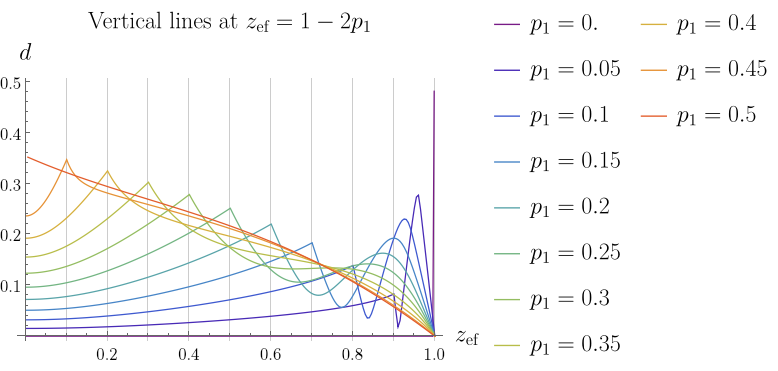
\includegraphics[width=0.9\linewidth]{appendices/figures/dist_avg_max_vs_z.png}
      \caption{Nueve no preferencial}
    \end{subfigure}%
    \begin{subfigure}{0.5\textwidth}
      \centering
      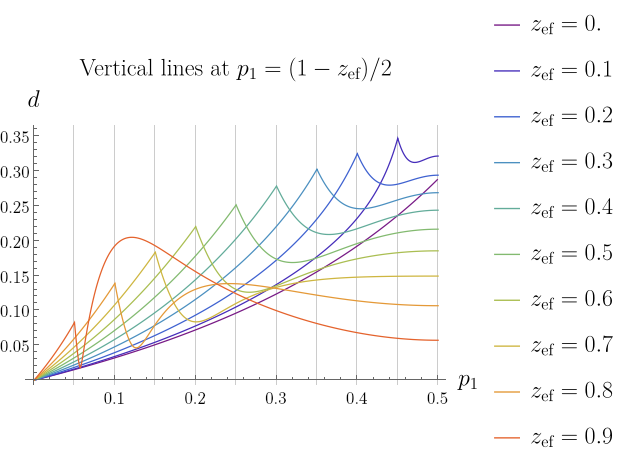
\includegraphics[width=0.9\linewidth]{appendices/figures/dist_avg_max_vs_p.png}
      \caption{Noventa y nueve partículas no preferenciales}
    \end{subfigure}
    \caption{Distancia entre asignaciones \acnote{Jjajaja tengo que arreglar esta figura}}\label{ap:DistAvgMaxEnt}
\end{figure}
La figura \ref{ap:DistAvgMaxEnt} revela que las asignaciones son iguales en el caso en el que $p_{1}=0$, así como cuando $r_{\ef}=1.$. En efecto, si el estado efectivo es puro, entonces \acnote{demostración de que son iguales}
\begin{align}
    lkjasdf
\end{align}
Además, se observan máximos locales en la distancia entre las asignaciones siempre que $p_{1}=\frac{1-r_{\ef}}{2}$. Esto es un resultado del comportamiento de la asignación promedio.

\section{Algunas dinámicas}

\subsection{Dinámicas factorizables}

\subsection{La compuerta SWAP}

\subsection{Canales de Pauli}

\section{Comparación de resultados de ambas asignaciones}